%%
% !authored by https://tingfengx.github.io/
%%
\documentclass{beamer}
\title{\LARGE{GOMOKU} \\ \small{Walk through and Final Report}}
\author{Lab 3165, Thursday Evenings @ Station 63/64}
\institute{University of Toronto}
\begin{document}
\maketitle

\newpage

\begin{frame}
    \frametitle{WHY GOMOKU?}
    Gomoku is a board game where each step is built upon previous choices which means to implement this game, we will need to store states. We will need to build a sequential circuit with registers. At the same time, the circuit will need to be clocked, which is again, related to CSC258 material. The game state(game board) will be displayed on a screen through a VGA cable and this is related to the Lab7 material. We will also use the hex display to show some of the stats for the ongoing game. 
\end{frame}




\begin{frame}
\frametitle{Project Milestones}

\begin{itemize}
    \item Display the empty board on the screen through VGA cable. Go over the resources posted on quercus regarding keyboard control and then implement the keyboard control. Find resources for the while/black token and the game board.\newline
    \item Users should be able to move the pointer around on the screen using the arrow keys on the keyboard. Users should also be able to put the token down (using the enter key on the keyboard) on any valid position on the game board. Notice that tokens have alternating colour, meaning that if the last token put down was a white one the next one should be black. \newline
    \item Check if the game has been won or not. If won, by which player. Display a message for who won the game. Make the hex display various game stats, including the current player identified by the player’s number.
\end{itemize}
\end{frame}

\begin{frame}
    \frametitle{Worth Mentioning Features}
    \begin{itemize}
        \item Support of keyboard control through the PS2 interface.
        \item Moving cursor on the screen to indicate the current location of the cursor. No more looking at hex and counting on the grid!
        \item Automatic alternating colour switching, avoids cheating in game.
        \item Placing a stone at an already occupied location is forbidden.
        \item Automatic judging of winner, more fair!
    \end{itemize}
\end{frame}

\begin{frame}
    \frametitle{Implementation Details}
    \framesubtitle{Structure of the project}
    \begin{itemize}
        \item \texttt{GOMOKU\_FPGA/adapters/*}
        \begin{itemize}
            \item Contains PS2 keyboard adapters, courtesy of Alex Hurka, link provided by professor on Quercus, under Project Proposal + Resources section. 
            \item Contains VGA Adapters, borrowed from Lab 7 of CSC258.
        \end{itemize}
        \item \texttt{GOMOKU\_FPGA/DE1\_SoC.qsf}
        \begin{itemize}
            \item Required pin assignment file for the FPGA board, provided by professor on Quercus.
        \end{itemize}
        \item \texttt{GOMOKU\_FPGA/gomoku.v}
        \begin{itemize}
            \item Actual Implementation of the Gomoku Game, top level instantiation name is \texttt{gomoku}. (This is code written by us. )
        \end{itemize}
        \item \texttt{GOMOKU\_FPGA/utils/*}
        \begin{itemize}
            \item Contains utility files, including the \texttt{bmp2mif} written in C provided.  
        \end{itemize}
    \end{itemize}
\end{frame}

\begin{frame}
    \frametitle{Implementation Details}
    \framesubtitle{Input using the PS2 Keyboard}
    \begin{itemize}
        \item \texttt{<space>} for starting the game
        \item \texttt{a} for moving toward left by one position
        \item \texttt{s} for moving down by one position
        \item \texttt{d} for moving right by one position
        \item \texttt{w} for moving up by one position
        \item \texttt{enter} for placing the stone at the position where the cursor is currently at.
        
    \end{itemize}
\end{frame}

\begin{frame}
    \frametitle{Implementation Details}
    \framesubtitle{Output Data on HEX and VGA display}
    \begin{itemize}
        \item \texttt{HEX0} for $y$ location on the grid, from 0 up to 6
        \item \texttt{HEX1} for $x$ location on the grid, from 0 up to 6
        \item \texttt{HEX4 \& HEX5} for the number of steps taken to win the game. Users can compare the number of steps taken to win the game!
    \end{itemize}
\end{frame}

\begin{frame}
    \frametitle{What did we do? (Main Components)}
    \framesubtitle{FSM that draws the screen}
    \center 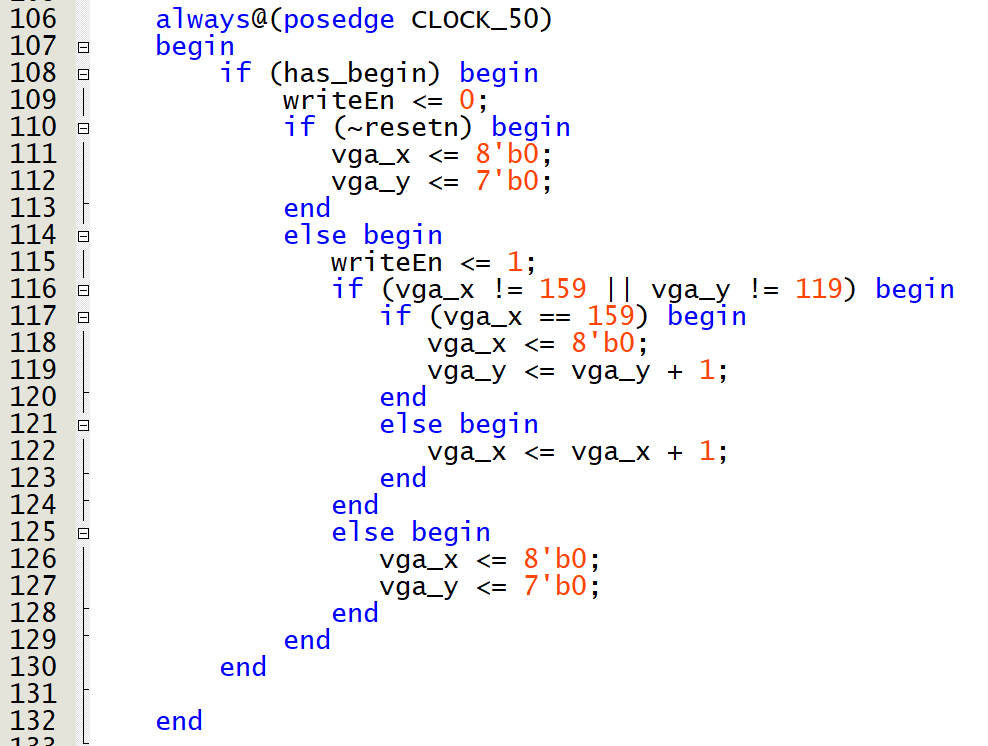
\includegraphics[scale=0.4]{screen_fsm.png}
\end{frame}

\begin{frame}
    \frametitle{What did we do? (Main Components)}
    \framesubtitle{Choosing the colour}
    \center 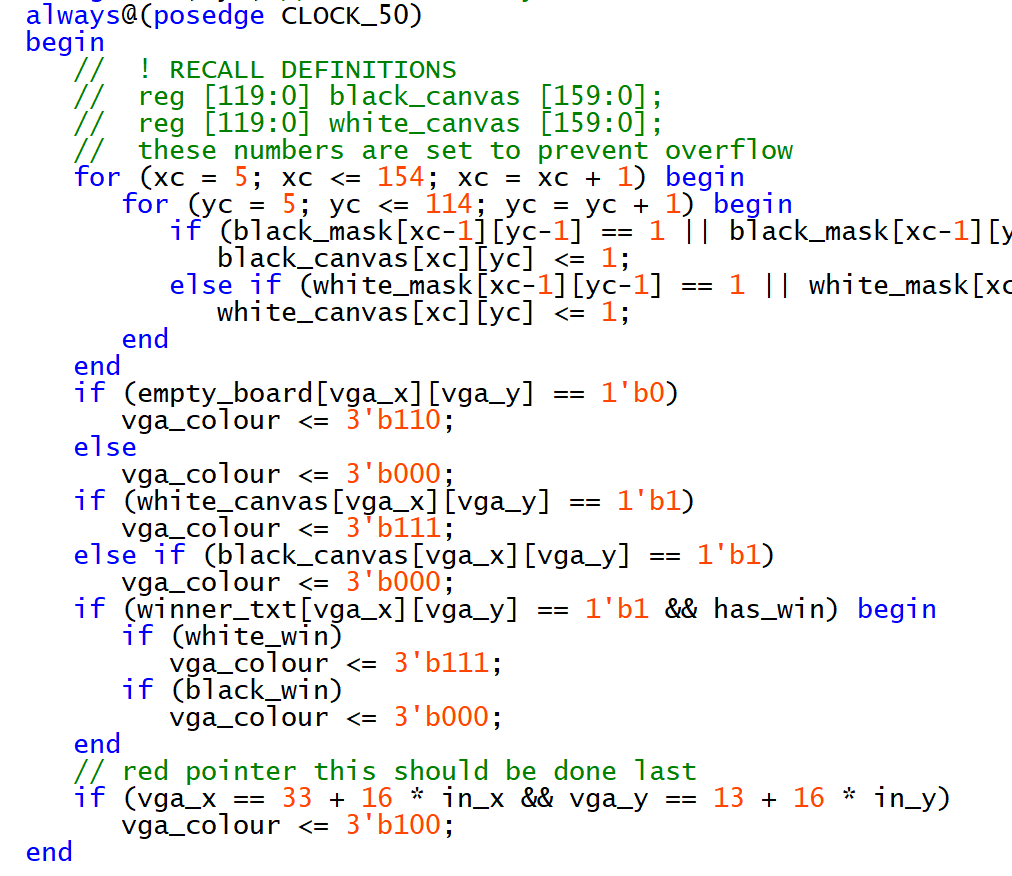
\includegraphics[scale=0.4]{color_fsm.png}
\end{frame}

\begin{frame}
    \frametitle{What did we do? (Main Components)}
    \framesubtitle{Keyboard Controller}
    \center 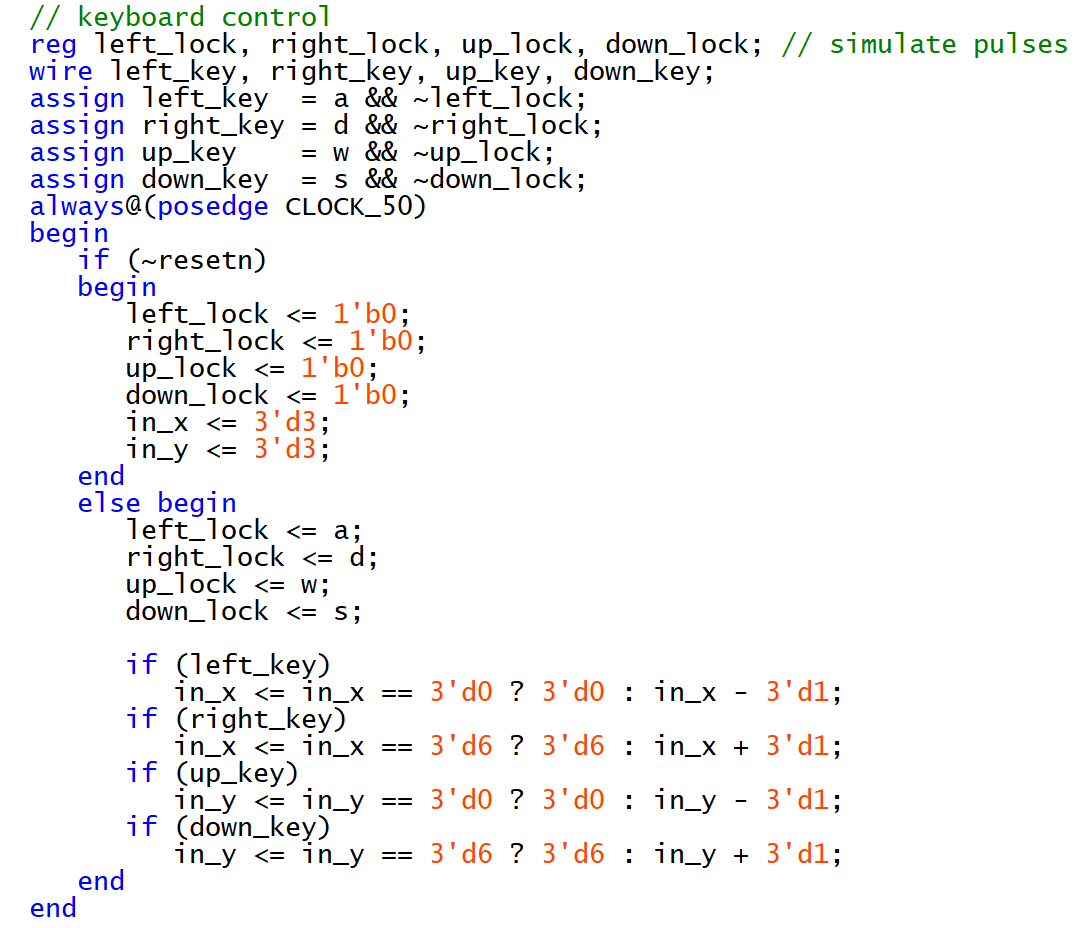
\includegraphics[scale=0.4]{keyboard.png}
\end{frame}

\begin{frame}
    \frametitle{What did we do? (Main Components)}
    \framesubtitle{Placing Stones}
    \center 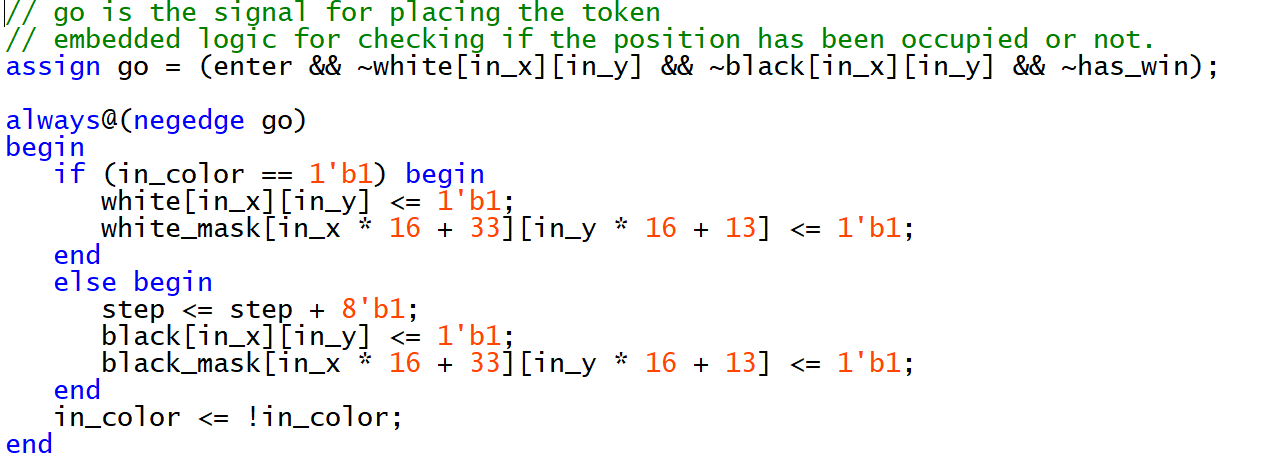
\includegraphics[scale=0.4]{place_go.png}
\end{frame}

\begin{frame}
    \frametitle{Discussion}
    \framesubtitle{Did it work?}
    \begin{itemize}
        \item Yes! It works well!
        \item Up to our manual testing by playing against each other there is no bug.
        \item We tested main components of the project using ModelSim and they behave exactly as what we want : p
    \end{itemize}
\end{frame}

\begin{frame}
    \frametitle{Discussion}
    \framesubtitle{What did you learn specifically}
    \begin{itemize}
        \item Keyboard Control! This was brand new to us and took a long time to figure out how to use the module. It is really cool to be able to control the game using a keyboard. 
        \item In lab7 we encountered the VGA module, however at that time we just followed the instructions and didn't really dive into how things were realized. After the project, we completely understood that VGA has to be drawn with two components, one moving the pointer to different positions and then one changing the colour as appropriate while we loop over the area that we want to draw. 
    \end{itemize}
\end{frame}

\begin{frame}
    \frametitle{Discussion}
    \framesubtitle{What did you learn specifically}
    \begin{itemize}
        \item Initial Blocks! This didn't appear in the course material but we find it was a great help in initializing the registers which we used to hold initial values needed for the program.
        \item For loops! This is not synthesis-able code, but it turns out to be very useful for handling code that are repetitive!
    \end{itemize}
\end{frame}

\begin{frame}
    \frametitle{Discussion}
    \framesubtitle{What would you do differently next time?}
    \begin{itemize}
    \item For a static game like this, maybe it is a better idea to have the screen not redrawn over and over : (
    \item To be more (computationally) efficient, we can try to figure out what part of the pixels change during each transition and just redraw/overwrite the specific part. 
    \item Use a memory map rather than using arrays to store information about the screen. 
    \end{itemize}
\end{frame}


\begin{frame}
    \frametitle{Conclusion}
    \begin{itemize}
        \item We think the project definitely helped us better understand the course materials and especially verilog!
        \item It is nice to see what we learnt in class in action using a cool project. 
        \item Until now, ModelSim is still not very intuitive to us and in that sense hardware has been hard for us. However, hardware has also been great fun!
        \item We are thankful to our TA who have been working diligently through out the term in making sure we understand key concepts through out the term. Thank you so much, we really appreciate it!
    \end{itemize}
\end{frame}

\begin{frame}
    \frametitle{}
    \center \LARGE Time for a little demo!
\end{frame}


\begin{frame}
    \frametitle{Start Screen}
    \center
    \includegraphics[scale=0.07]{start.jpeg}
\end{frame}

\begin{frame}
    \frametitle{Game Play and Win!!}
    \center
    \includegraphics[scale=0.07]{gameplay.jpeg}
\end{frame}


\end{document}
